\section{Sơ đồ Activity}

\subsection{Sơ đồ activity về chức năng xác thực}
\begin{figure}[H]
    \centering
    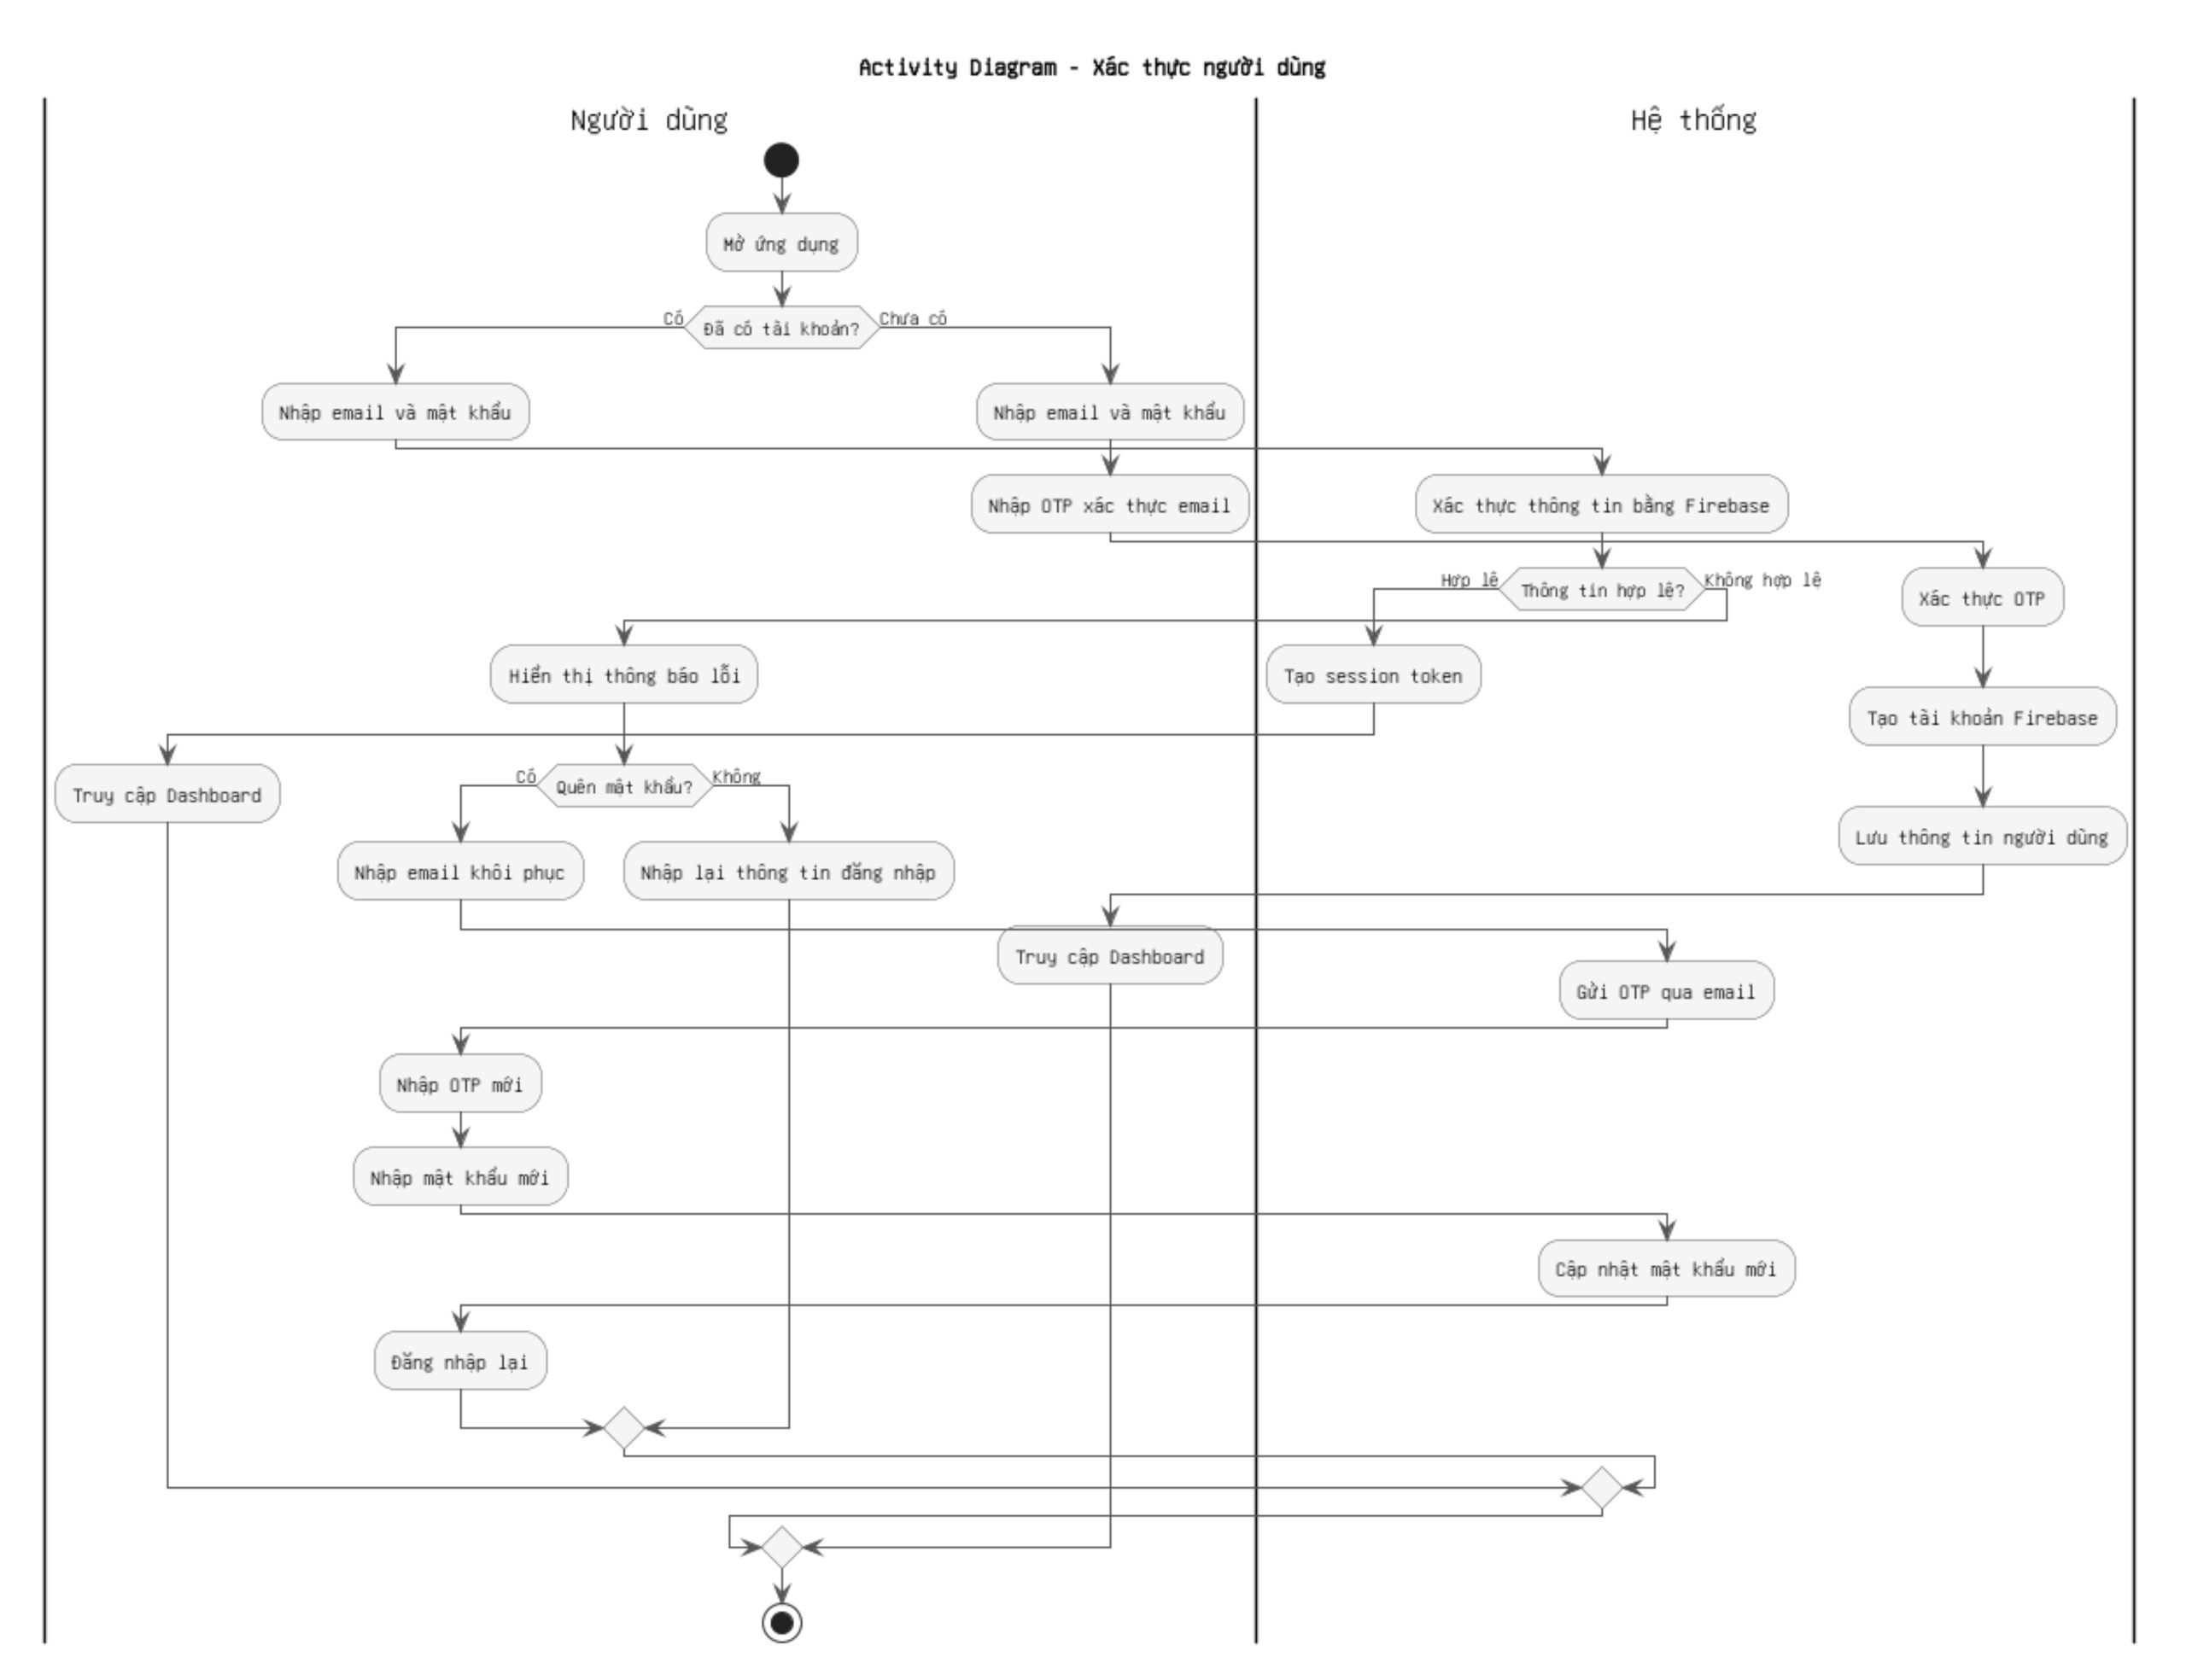
\includegraphics[width=1.0\textwidth]{figures/acti_xac_thu.jpg}
    \caption{Sơ đồ Activity về chức năng xác thực}
    \label{fig:activity_xac_thuc}
\end{figure}


Sơ đồ activity ở Hình~\ref{fig:activity_xac_thuc} mô tả luồng xử lý chức năng xác thực người dùng,
bao gồm hai tác nhân chính là \textbf{Người dùng} và \textbf{Hệ thống}. Luồng hoạt động được
chia thành hai nhánh chính tùy theo trạng thái tài khoản của người dùng.

\textbf{Trường hợp đã có tài khoản:} Người dùng nhập email và mật khẩu, hệ thống tiến hành
xác thực thông tin thông qua Firebase. Nếu thông tin hợp lệ, hệ thống tạo session token và
cho phép người dùng truy cập Dashboard. Ngược lại, hệ thống hiển thị thông báo lỗi và người
dùng có thể chọn nhập lại thông tin hoặc thực hiện khôi phục mật khẩu. Trong luồng khôi phục,
người dùng nhập email để nhận OTP, sau đó đặt mật khẩu mới và tiến hành đăng nhập lại.

\textbf{Trường hợp chưa có tài khoản:} Người dùng nhập email, mật khẩu và OTP xác thực
email. Hệ thống lần lượt xác thực OTP, tạo tài khoản trên Firebase và lưu thông tin người dùng,
sau đó cho phép truy cập Dashboard.

\subsection{Sơ đồ activity về chức năng phát hiện té ngã}
\begin{figure}[H]
    \centering
    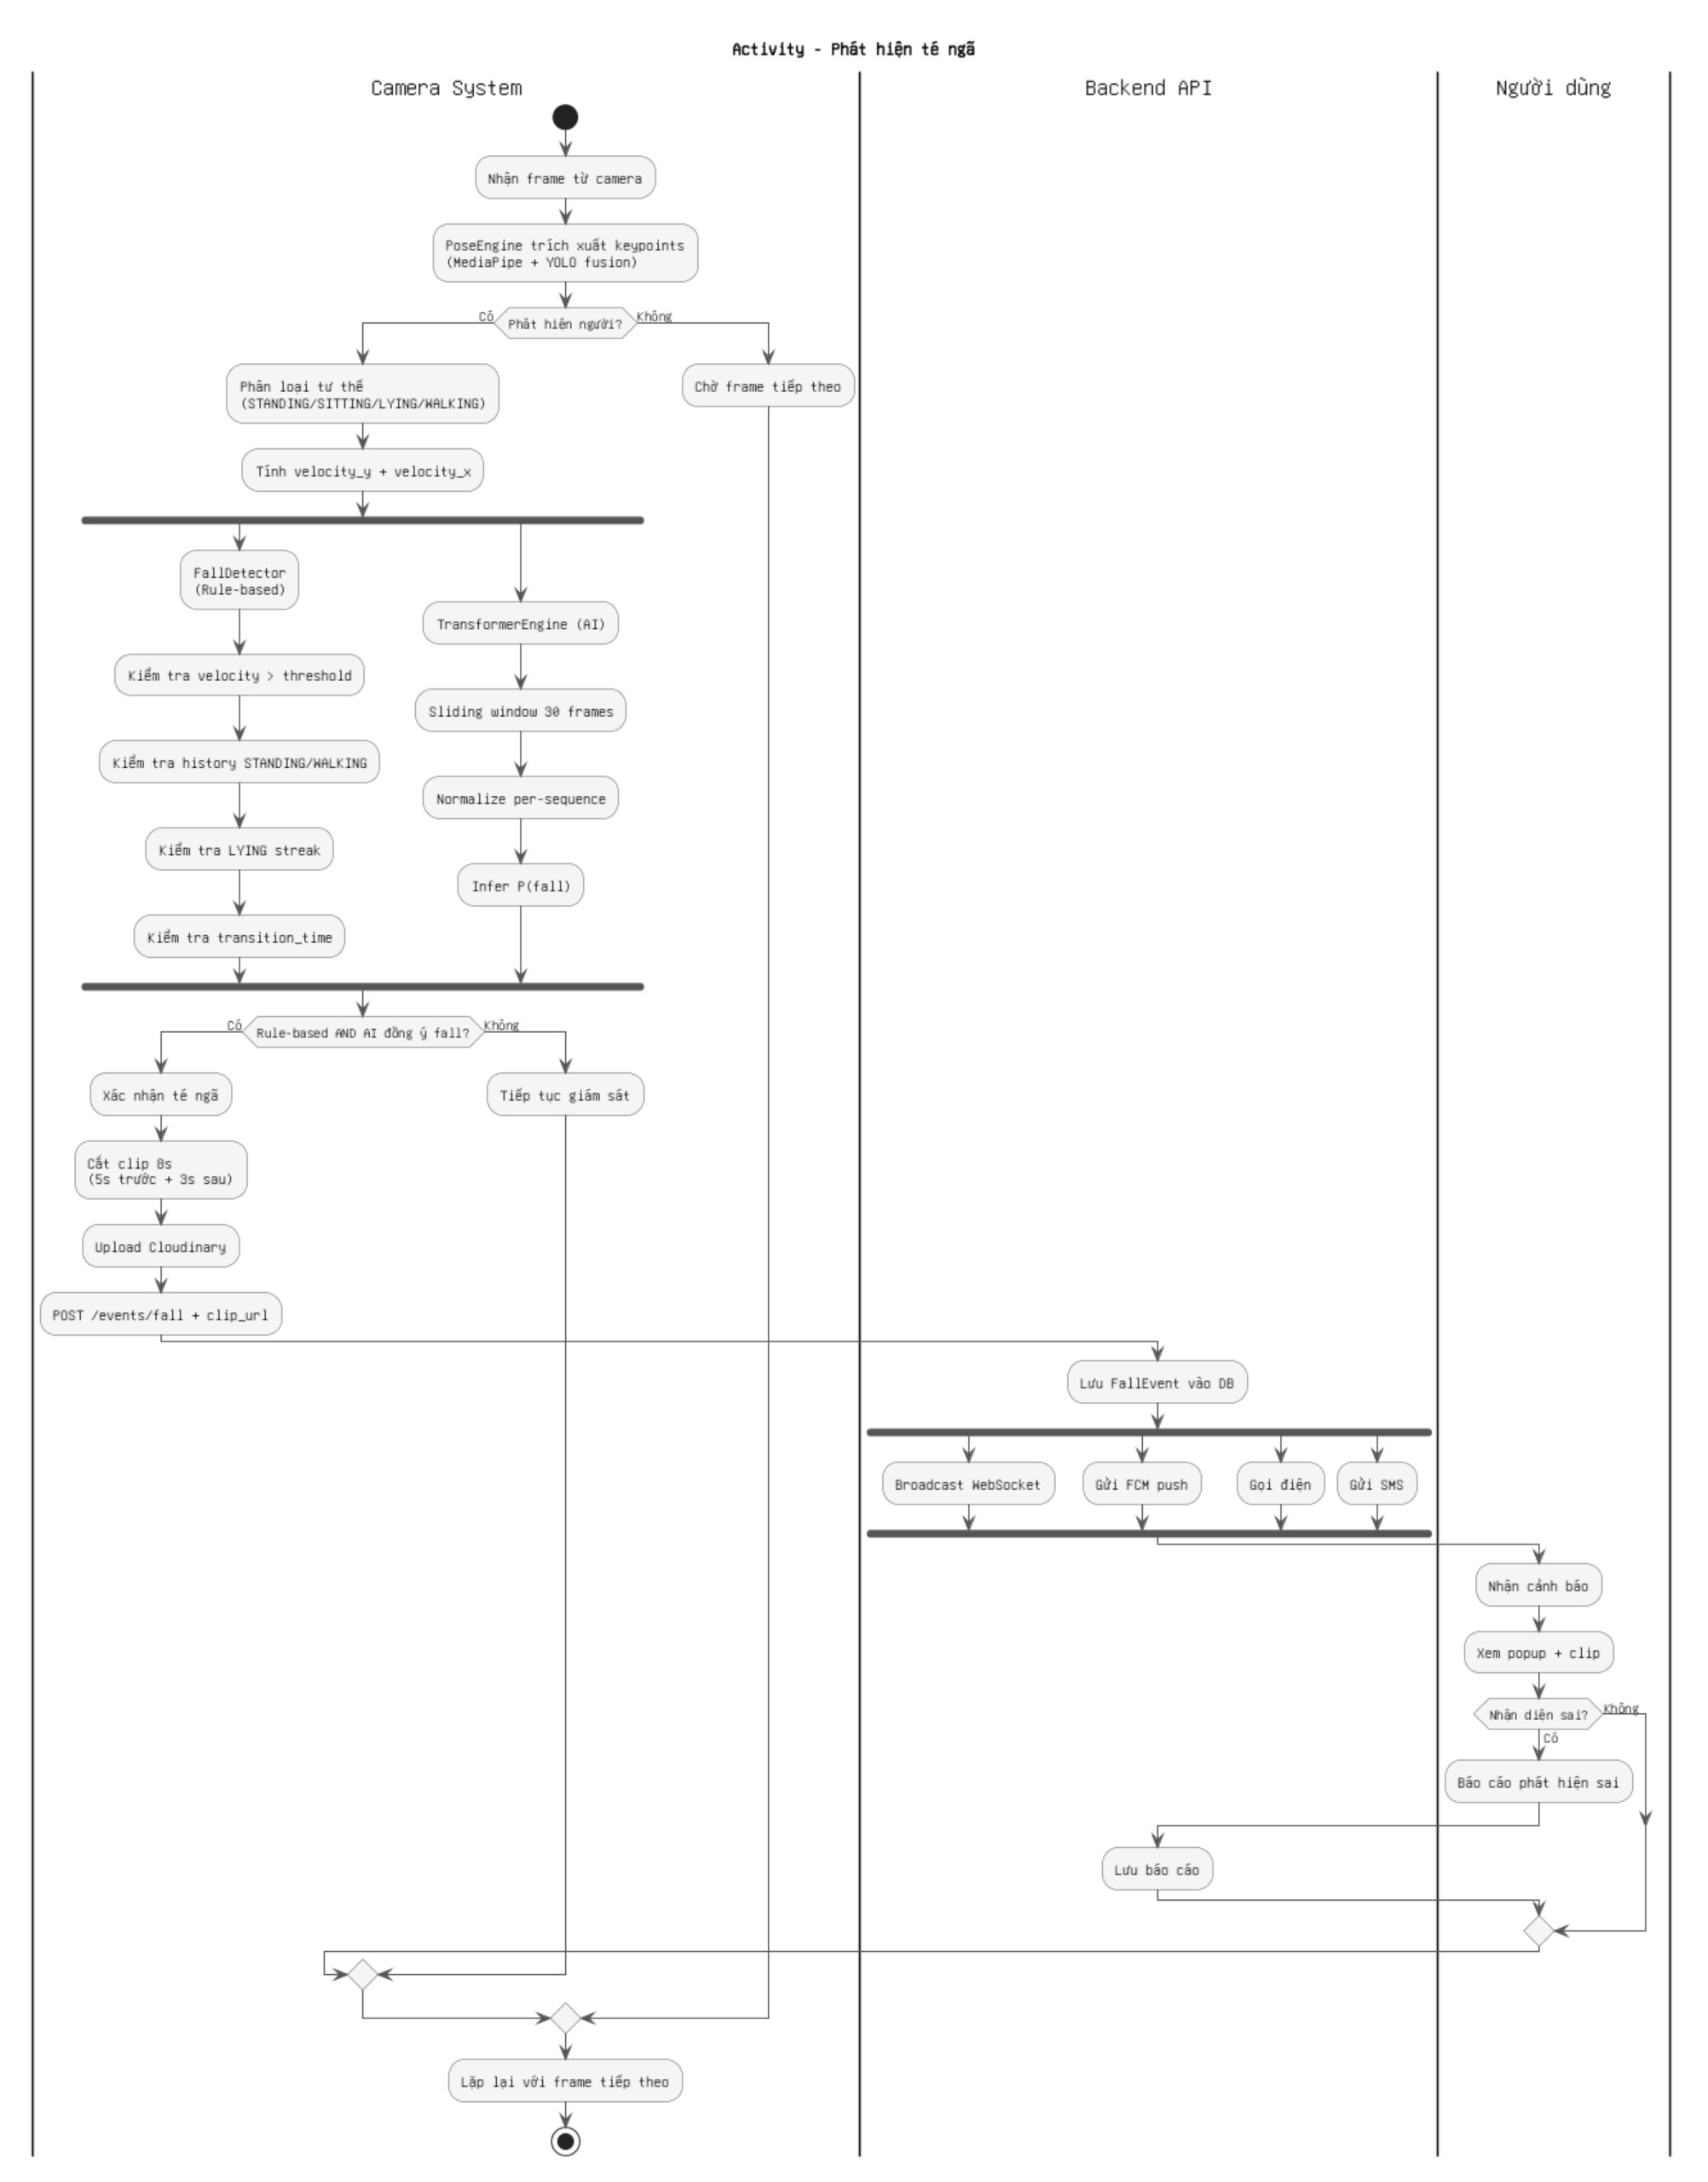
\includegraphics[width=0.8\textwidth]{figures/acti_phat_hien.jpg}
    \caption{Sơ đồ Activity về chức năng phát hiện té ngã}
    \label{fig:activity_phat_hien}
\end{figure}

Sơ đồ activity ở Hình~\ref{fig:activity_phat_hien} mô tả luồng xử lý chức năng phát hiện
té ngã theo thời gian thực, với sự phối hợp giữa ba tác nhân: Camera System,
Backend API và Người dùng.

\textbf{Giai đoạn trích xuất và phân tích tư thế:} Hệ thống liên tục nhận frame từ camera
và sử dụng PoseEngine -- kết hợp MediaPipe và YOLO -- để trích xuất keypoints của người
trong khung hình. Nếu phát hiện có người, hệ thống phân loại tư thế hiện tại
(STANDING, SITTING, LYING, WALKING) đồng thời tính toán vận tốc theo trục $x$ và $y$.

\textbf{Giai đoạn phát hiện té ngã song song:} Hệ thống thực hiện đồng thời hai cơ chế
phát hiện. Thứ nhất, FallDetector dựa trên tập luật (rule-based) kiểm tra các
điều kiện gồm ngưỡng vận tốc, lịch sử tư thế, số frame liên tiếp ở trạng thái LYING
và thời gian chuyển tiếp giữa các tư thế. Thứ hai, TransformerEngine sử dụng
mô hình AI với cửa sổ trượt 30 frame, chuẩn hóa dữ liệu theo chuỗi và suy luận xác suất
té ngã $P(\text{fall})$.

\textbf{Giai đoạn xác nhận và cảnh báo:} Té ngã chỉ được xác nhận khi cả hai cơ chế
đồng thời cho kết quả dương tính. Khi đó, hệ thống cắt đoạn clip 6 giây (3 giây trước
và 3 giây sau sự kiện), tải lên Cloudinary và gửi thông tin đến Backend API để lưu vào
cơ sở dữ liệu. Cảnh báo được phát đồng thời qua bốn kênh: WebSocket, thông báo đẩy FCM,
cuộc gọi điện thoại và tin nhắn SMS.

\textbf{Giai đoạn phản hồi của người dùng:} Sau khi nhận cảnh báo, người dùng có thể
xem popup kèm clip sự kiện. Nếu phát hiện là sai, người dùng có thể gửi báo cáo để
hệ thống lưu lại nhằm cải thiện độ chính xác. Trong trường hợp không phát hiện té ngã,
hệ thống tiếp tục vòng lặp giám sát với frame tiếp theo.

\subsection{Sơ đồ activity về chức năng nhận diện khuôn mặt và thông báo tư thế}
\begin{figure}[H]
    \centering
    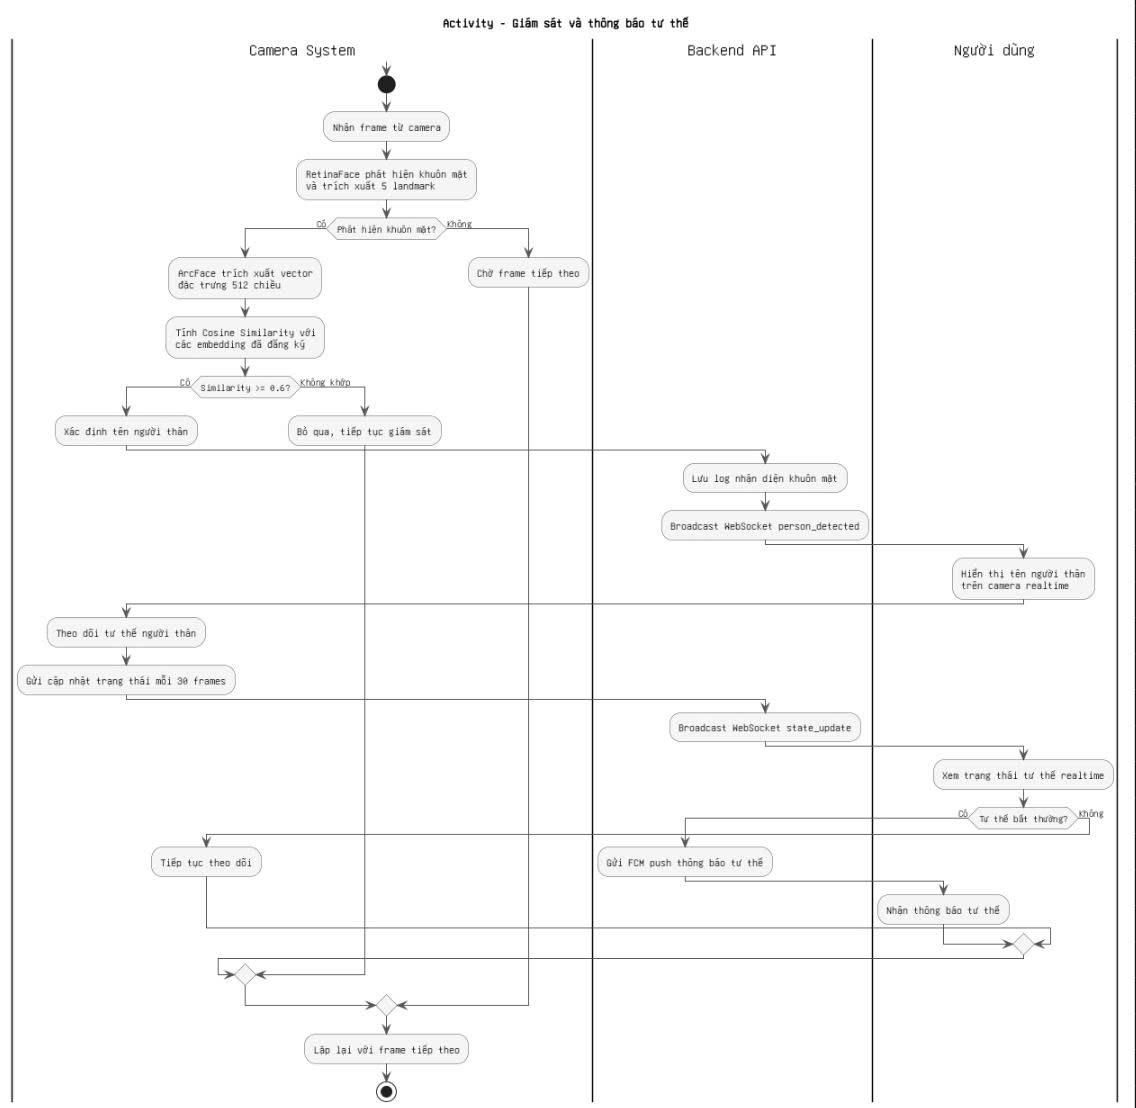
\includegraphics[width=0.8\textwidth]{figures/ac_face.jpg}
    \caption{Sơ đồ Activity về chức năng nhận diện khuôn mặt và thông báo tư thế}
    \label{fig:activity_nhan_dien_khuon_mat}
\end{figure}

Sơ đồ activity ở Hình~\ref{fig:activity_nhan_dien_khuon_mat} mô tả luồng xử lý chức năng
giám sát tư thế và thông báo, với sự tham gia của ba tác nhân: Camera System, Backend API
và Người dùng. Face embedding sử dụng trong luồng này được chuẩn bị sẵn từ luồng đăng ký
người thân.

Camera System liên tục nhận frame và sử dụng RetinaFace để phát hiện khuôn mặt cùng với
5 điểm landmark. Khi phát hiện được khuôn mặt, ArcFace trích xuất vector đặc trưng 512
chiều và tính Cosine Similarity với các embedding đã đăng ký. Nếu độ tương đồng đạt ngưỡng
$\text{sim} \geq 0{,}6$, hệ thống xác định danh tính người thân và ghi log nhận diện vào
cơ sở dữ liệu, đồng thời phát tín hiệu qua WebSocket để hiển thị tên người thân trực tiếp
trên giao diện camera của người dùng.

Hệ thống tiếp tục theo dõi tư thế của người thân và gửi cập nhật trạng thái mỗi 30 frame,
giúp người dùng quan sát trạng thái tư thế theo thời gian thực. Nếu phát hiện tư thế bất
thường, Backend API gửi thông báo đẩy FCM đến người dùng. Trong trường hợp khuôn mặt không
đạt ngưỡng tương đồng hoặc không phát hiện được khuôn mặt, hệ thống bỏ qua và tiếp tục
giám sát frame tiếp theo.
\subsection{Sơ đồ activity về chức năng lưu lịch sử}
\begin{figure}[H]
    \centering
    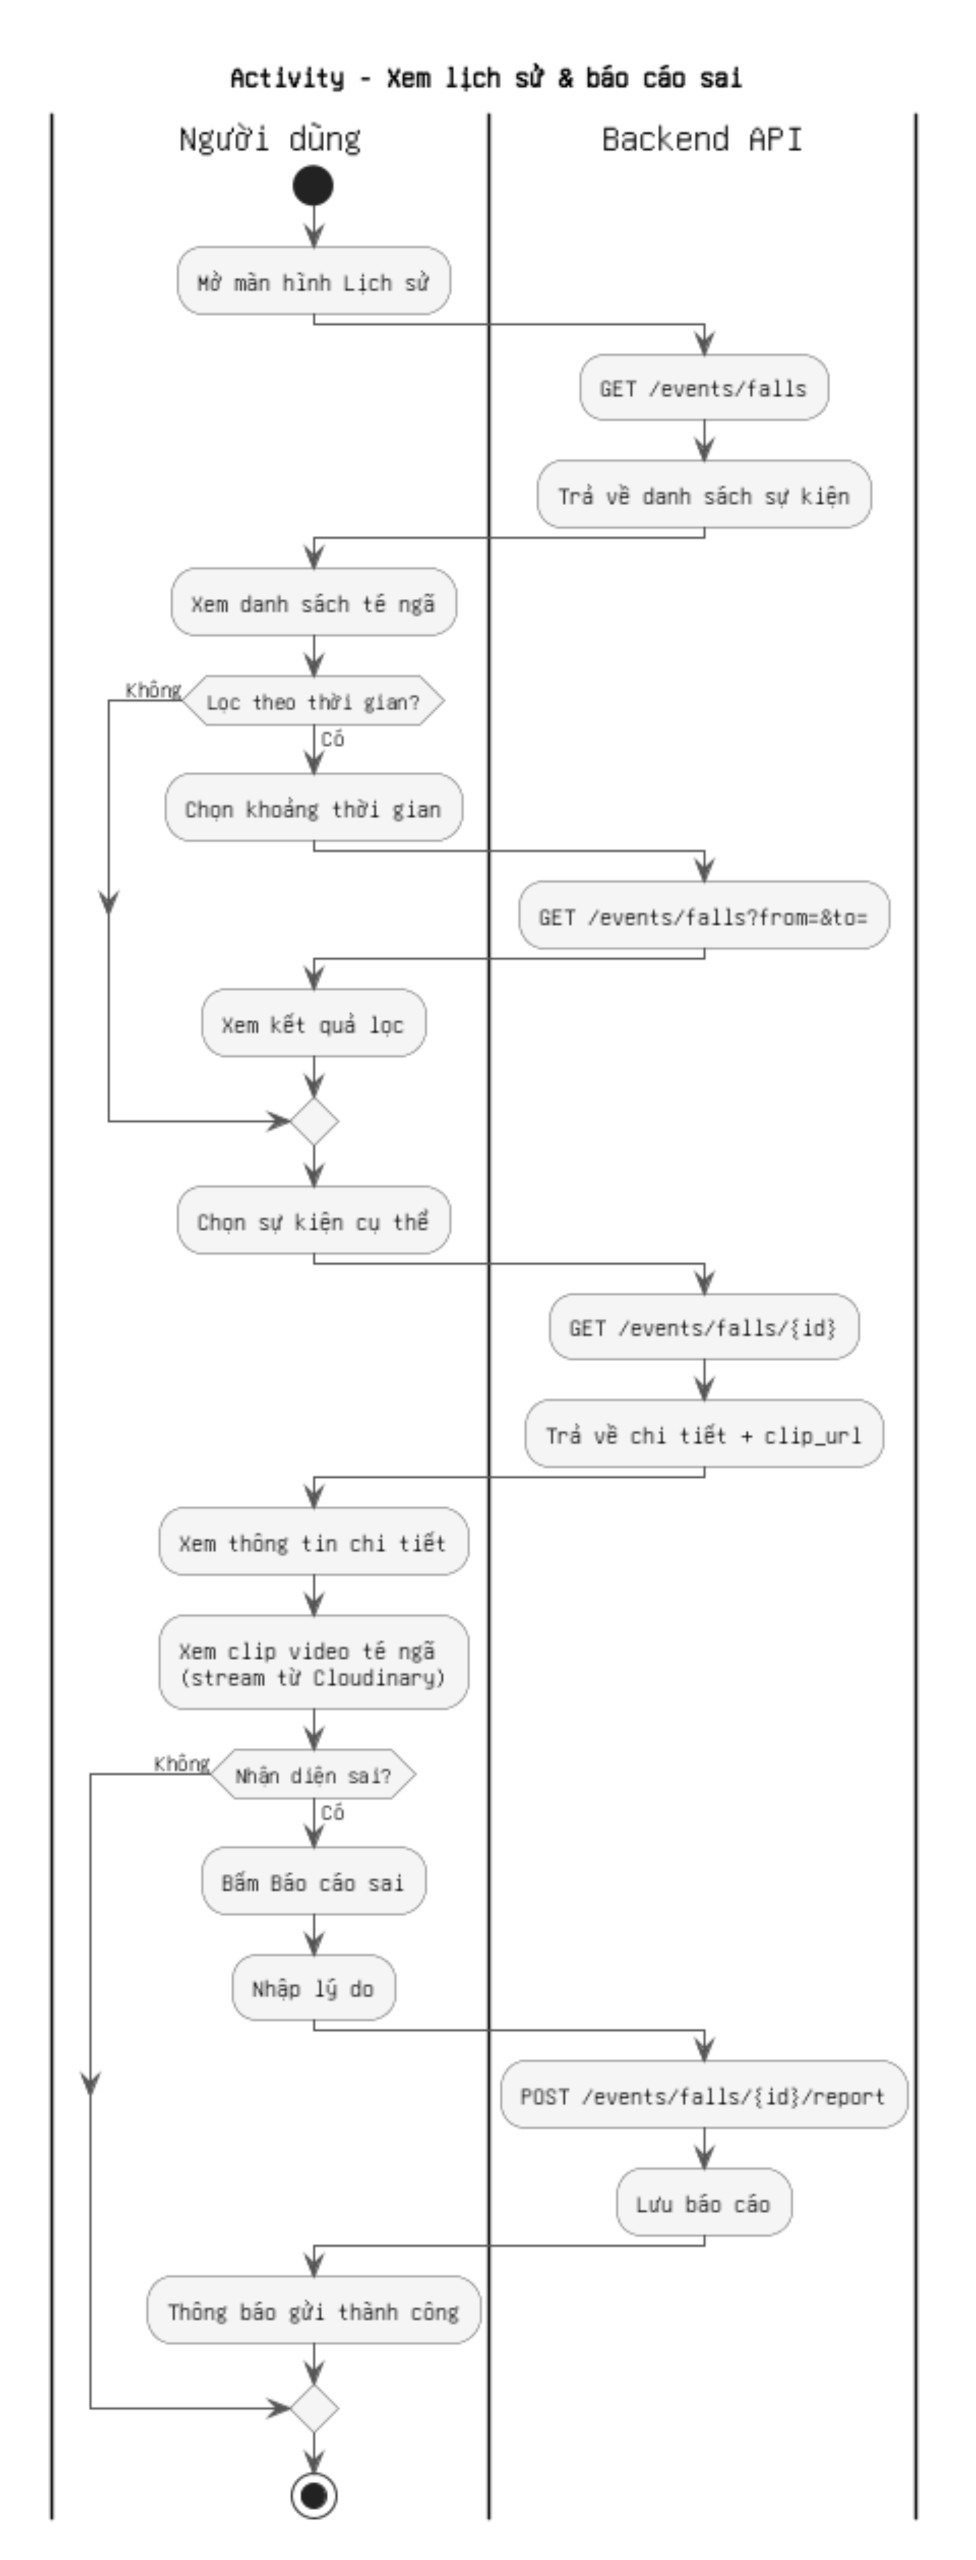
\includegraphics[width=0.5\textwidth]{figures/ac_xem_ls_report.jpg}
    \caption{Sơ đồ Activity về chức năng lưu lịch sử}
    \label{fig:activity_lich_su}
\end{figure}

Sơ đồ activity ở Hình~\ref{fig:activity_lich_su} mô tả luồng xử lý chức năng xem lịch
sử té ngã và báo cáo nhận diện sai, với sự tham gia của hai tác nhân: Người dùng và
Backend API.

Người dùng mở màn hình Lịch sử, Backend API truy vấn và trả về danh sách các sự kiện
té ngã qua GET /events/falls. Người dùng có thể lọc danh sách theo khoảng thời
gian mong muốn, khi đó Backend API thực hiện truy vấn có tham số \texttt{from} và
\texttt{to} để trả về kết quả tương ứng.

Sau khi chọn một sự kiện cụ thể, Backend API trả về thông tin chi tiết kèm theo
clip\_url qua GET /events/falls/\{id\}. Người dùng có thể xem thông tin chi
tiết và xem lại clip video té ngã được stream trực tiếp từ Cloudinary.

Nếu người dùng nhận thấy sự kiện bị nhận diện sai, họ có thể bấm báo cáo sai và nhập
lý do. Backend API tiếp nhận báo cáo qua POST /events/falls/\{id\}/report và
lưu vào cơ sở dữ liệu. Báo cáo này sau đó sẽ được Web Admin xem xét và duyệt trong
luồng xử lý riêng. Người dùng nhận được thông báo gửi báo cáo thành công.

\subsection{Sơ đồ activity về chức năng xử lý thông báo}
\begin{figure}[H]
    \centering
    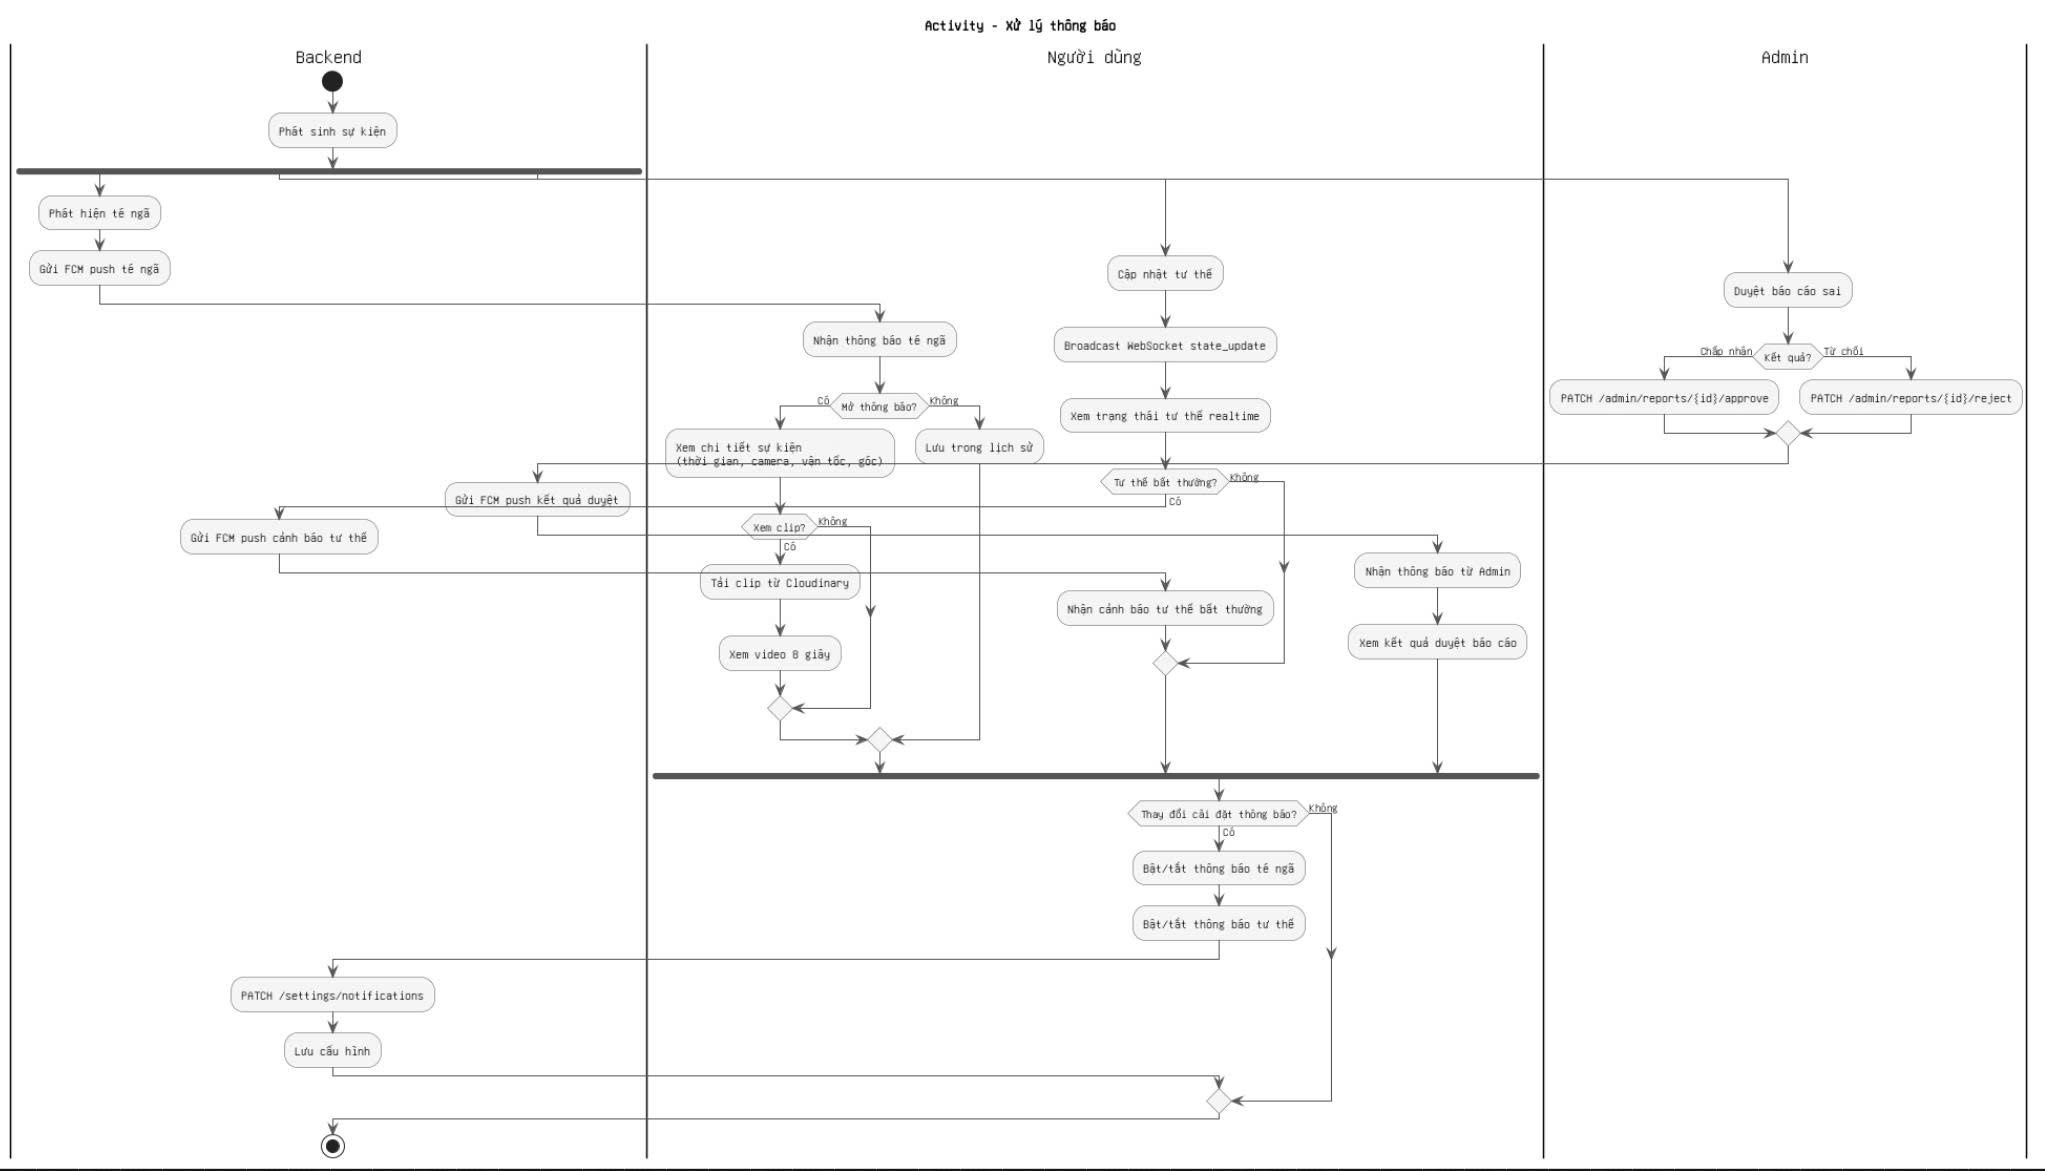
\includegraphics[width=1.0\textwidth]{figures/ac_thong_bao.jpg}
    \caption{Sơ đồ Activity về chức năng xử lý thông báo}
    \label{fig:activity_thong_bao}
\end{figure}

Sơ đồ activity ở Hình~\ref{fig:activity_thong_bao} mô tả luồng xử lý thông báo,
với sự tham gia của ba tác nhân: Backend, Admin và Người dùng. Hệ thống xử lý
đồng thời ba luồng thông báo độc lập nhau.

Luồng thứ nhất là thông báo té ngã. Backend gửi FCM push khi phát hiện sự kiện
té ngã. Nếu người dùng mở thông báo, ứng dụng hiển thị chi tiết sự kiện gồm thời
gian, camera, vận tốc và góc cơ thể. Người dùng có thể xem thêm clip video 6 giây
được tải từ Cloudinary. Nếu không mở, thông báo được lưu trong danh sách lịch sử.

Luồng thứ hai là thông báo tư thế. Backend liên tục broadcast trạng thái tư thế
qua WebSocket để người dùng theo dõi realtime. Khi phát hiện tư thế bất thường,
Backend gửi thêm FCM push cảnh báo đến người dùng.

Luồng thứ ba là thông báo từ Admin. Sau khi Admin duyệt chấp nhận hoặc từ chối
báo cáo sai, Backend gửi FCM push kết quả đến người dùng liên quan để xem kết
quả xử lý.

Ngoài ra, người dùng có thể vào cài đặt để bật hoặc tắt từng loại thông báo,
cấu hình được lưu lại qua PATCH /settings/notifications.



\subsection{Sơ đồ activity về chức năng  đăng ký theo dõi người thân}
\begin{figure}[H]
    \centering
    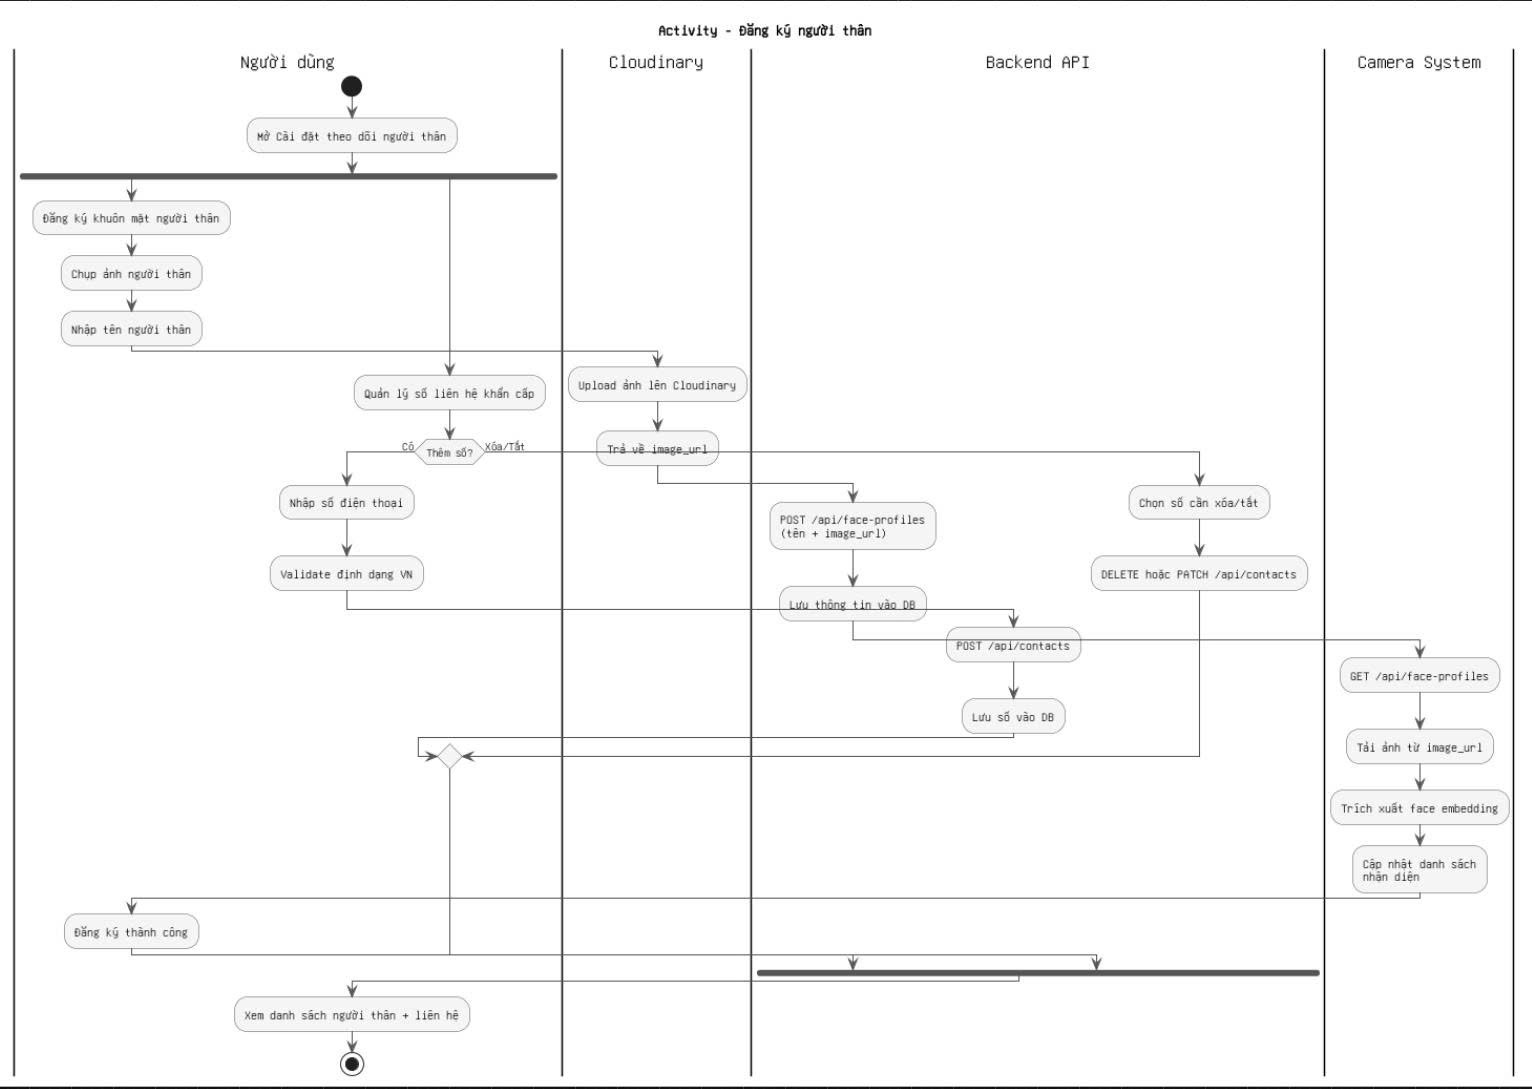
\includegraphics[width=1.0\textwidth]{figures/ac_theo_doi.jpg}
    \caption{Sơ đồ Activity về chức năng đăng ký theo dõi người thân}
    \label{fig:activity_theo_doi_nguoi_than}
\end{figure}


Sơ đồ activity ở Hình~\ref{fig:activity_theo_doi_nguoi_than} mô tả luồng xử lý chức năng
đăng ký người thân, với sự tham gia của bốn tác nhân: Người dùng, Cloudinary, Backend API
và Camera System.

Người dùng mở màn hình cài đặt theo dõi người thân và thực hiện đồng thời hai nhóm thao
tác độc lập nhau. Nhóm thứ nhất là đăng ký khuôn mặt người thân: người dùng chụp ảnh và
nhập tên người thân trên ứng dụng mobile, ảnh được upload lên Cloudinary và nhận về
image\_url. Backend API nhận thông tin gồm tên và image\_url qua POST /api/face-profiles
rồi lưu vào cơ sở dữ liệu. Camera System sau đó chủ động gọi GET /api/face-profiles
để tải ảnh, trích xuất face embedding và cập nhật danh sách nhận diện, sẵn sàng cho quá
trình giám sát. Nhóm thứ hai là quản lý số liên hệ khẩn cấp: người dùng có thể thêm số
điện thoại mới (có kiểm tra định dạng Việt Nam) hoặc xóa, tắt số đã có thông qua các
endpoint tương ứng trên Backend API.

Sau khi hoàn tất cả hai nhóm thao tác, người dùng có thể xem danh sách người thân và số
liên hệ đã đăng ký.

\subsection{Sơ đồ activity về chức năng tuỳ chỉnh camera}
\begin{figure}[H]
    \centering
    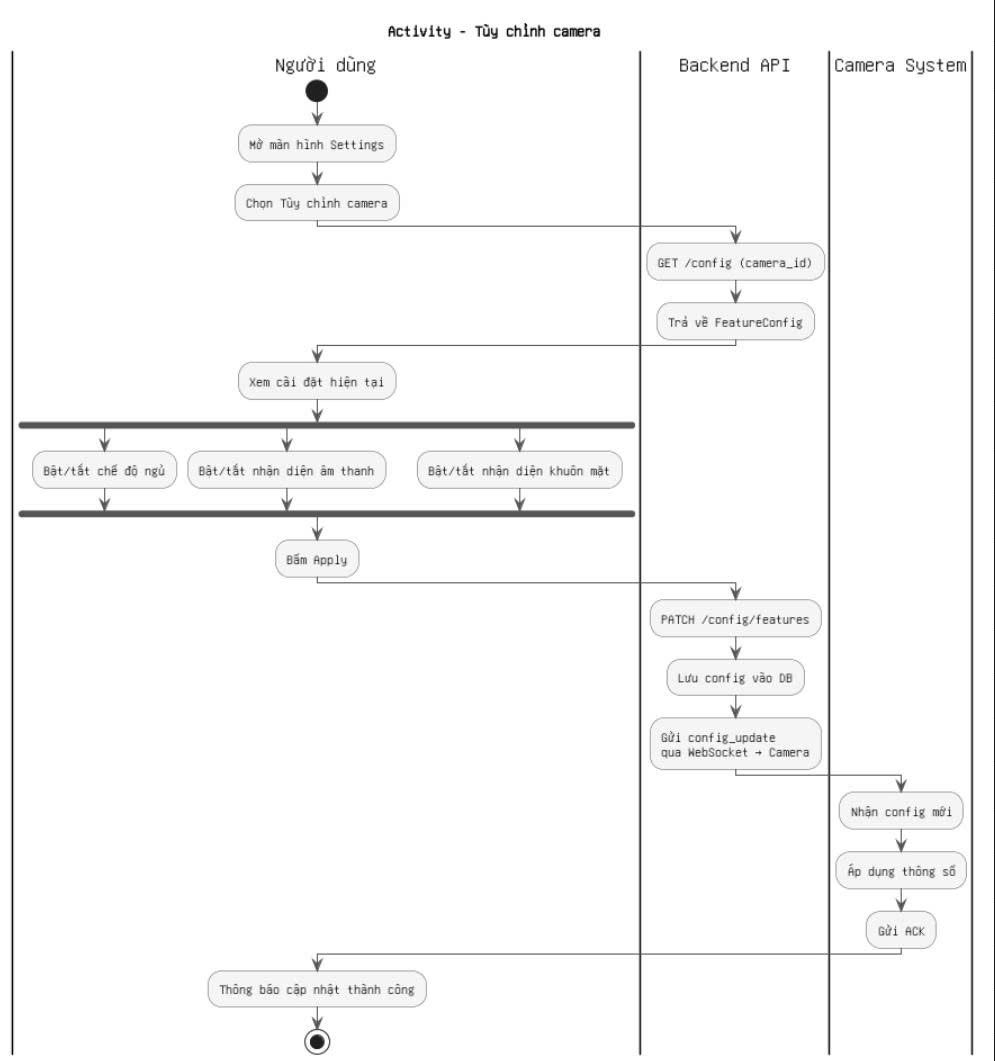
\includegraphics[width=0.8\textwidth]{figures/ac_tuy_chinh.jpg}
    \caption{Sơ đồ Activity về chức năng tuỳ chỉnh camera}
    \label{fig:activity_tuy_chinh_camera}
\end{figure}

Sơ đồ activity ở Hình~\ref{fig:activity_tuy_chinh_camera} mô tả luồng xử lý chức năng
tùy chỉnh camera, với sự tham gia của ba tác nhân: Người dùng, Backend API và Camera System.

Người dùng mở màn hình Settings và chọn chức năng tùy chỉnh camera. Backend API truy vấn
và trả về cấu hình chức năng hiện tại (FeatureConfig), cho phép người dùng xem các tùy
chọn đang được áp dụng.

Người dùng thực hiện đồng thời ba tùy chỉnh chức năng độc lập nhau, bao gồm bật/tắt chế
độ ngủ, bật/tắt nhận diện âm thanh và bật/tắt nhận diện khuôn mặt. Sau khi hoàn tất,
người dùng bấm Apply để xác nhận thay đổi.

Backend API cập nhật cấu hình qua PATCH /config/features, lưu vào cơ sở dữ liệu
và gửi sự kiện config\_update đến Camera System qua WebSocket. Camera System nhận cấu hình
mới, áp dụng các thông số và gửi ACK xác nhận. Người dùng nhận được thông báo cập nhật
thành công.


\subsection{Sơ đồ activity về chức năng quản lý hệ thống của Admin}
\begin{figure}[H]
    \centering
    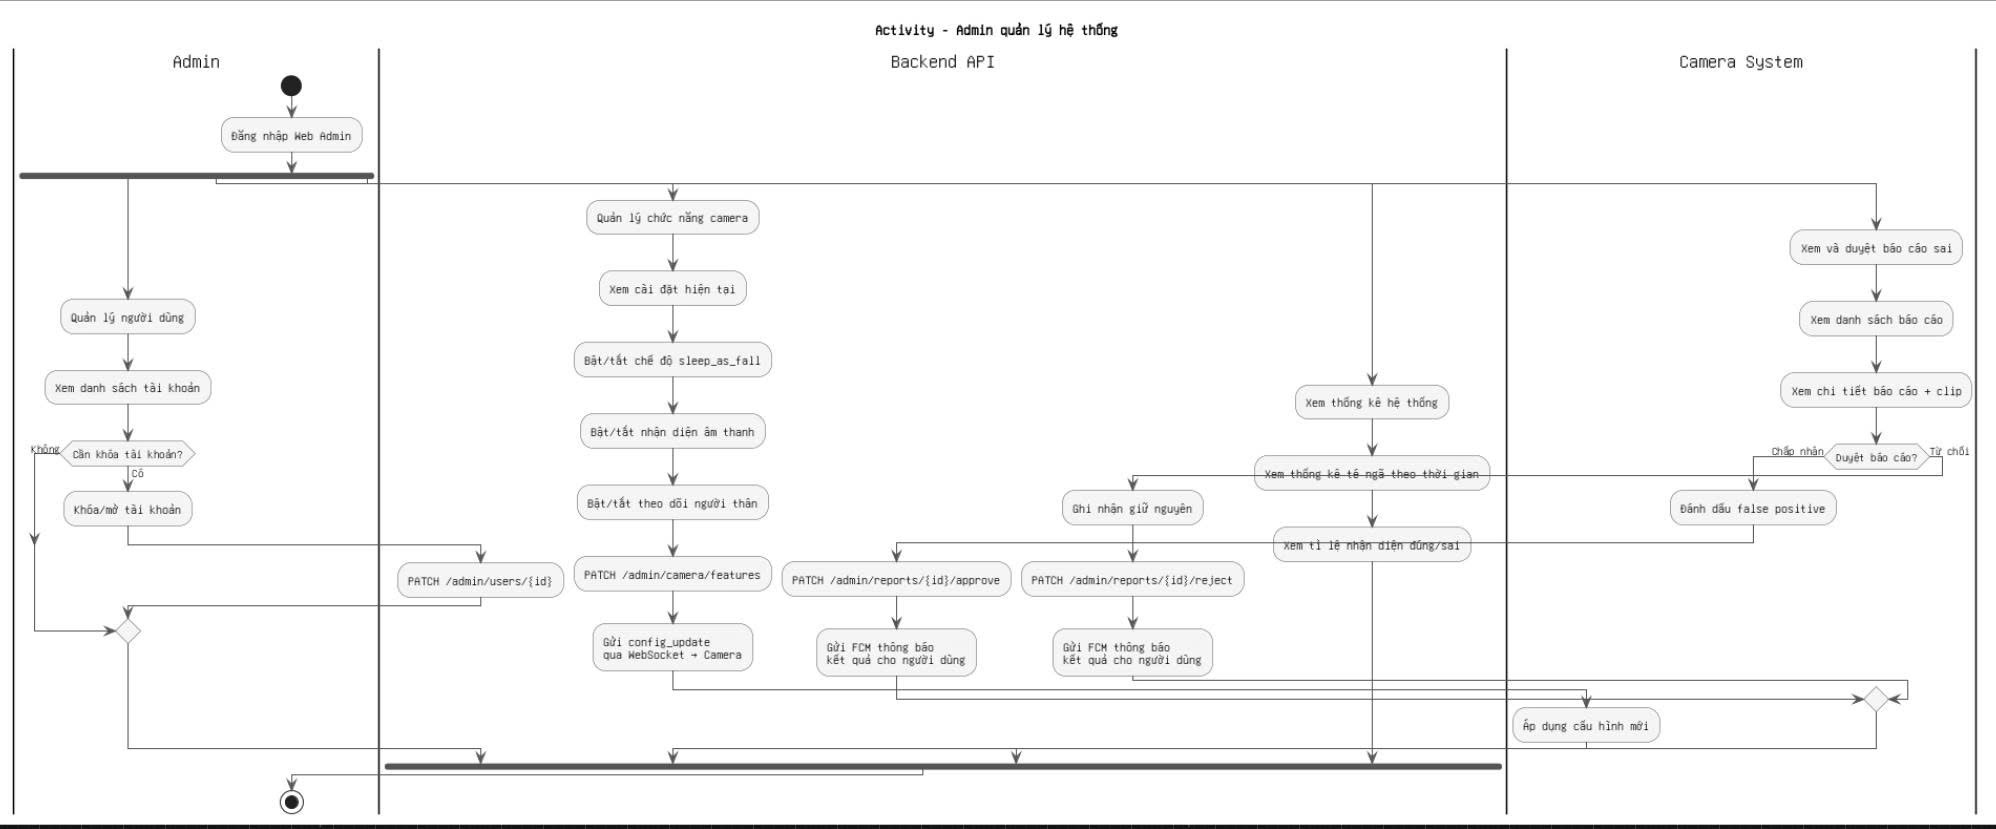
\includegraphics[width=1.0\textwidth]{figures/ac_admin.jpg}
    \caption{Sơ đồ Activity về chức năng quản lý hệ thống của Admin}
    \label{fig:activity_admin}
\end{figure}


Sơ đồ activity ở Hình~\ref{fig:activity_admin} mô tả luồng xử lý chức năng quản lý hệ
thống của Admin trên Web Admin, với sự tham gia của ba tác nhân: Admin, Backend API và
Camera System. Sau khi đăng nhập, Admin có thể thực hiện đồng thời bốn nhóm chức năng
độc lập nhau.

Nhóm thứ nhất là quản lý người dùng. Admin xem danh sách tài khoản và có thể khóa hoặc
mở khóa tài khoản khi cần thiết thông qua PATCH /admin/users/\{id\}.

Nhóm thứ hai là quản lý chức năng camera. Admin xem cài đặt hiện tại và thực hiện
bật hoặc tắt các chức năng gồm chế độ sleep\_as\_fall, nhận diện âm thanh và theo dõi
người thân. Backend API cập nhật cấu hình qua PATCH /admin/camera/features và
gửi config\_update đến Camera System qua WebSocket để áp dụng ngay lập tức.

Nhóm thứ ba là xem và duyệt báo cáo sai. Admin xem danh sách báo cáo từ người dùng,
xem chi tiết kèm clip video và đưa ra quyết định. Nếu chấp nhận báo cáo, sự kiện được
đánh dấu là false positive qua PATCH /admin/reports/\{id\}/approve. Nếu từ
chối, hệ thống ghi nhận giữ nguyên qua PATCH /admin/reports/\{id\}/reject.
Trong cả hai trường hợp, Backend API đều gửi thông báo FCM về kết quả duyệt đến người
dùng mobile.

Nhóm thứ tư là xem thống kê hệ thống. Admin có thể theo dõi thống kê số lượng sự kiện
té ngã theo thời gian và tỉ lệ nhận diện đúng so với sai, phục vụ việc đánh giá hiệu
quả hoạt động của hệ thống.